\section{Plan de implantación}
\par En esta sección se describirá el método de implantación del portal LifeRay 7 en un entorno de producción, de forma que sea integrable con otras instancias de LifeRay.

\subsection{Instalación del Software}
\par Antes de configurar el portal, será necesario instalarlo en el caso de que éste no se encuentre en el sistema. Para instalarlo, se utilizarán los siguientes componentes de software:
\begin{itemize}[-]
    \item LifeRay 7 con Tomcat 8: Web de Descarga
    \item Linux (recomendable que sea una distribución RHEL): Web de Descarga
    \item Oracle Java 8 JDK: Web de Descarga
\end{itemize}
\par Debido al carácter del documento, no se cubrirá cómo instalar el sistema operativo.

\subsection{Instalación de Java 8 JDK}
\par Desde la web de descarga, se deberá descargar el archivo RPM en el caso de utilizar una distribución RHEL o el archivo comprimido en el caso contrario. Para que la guía de implantación sea aplicable a cualquier distribución, se utilizará el archivo comprimido.
Primero se deberá extraer (recomendable extraerlo en \textit{/opt/ o en /usr/share}):

\begin{listing}[style=consola, numbers=none]
> tar xvf jdk.tar.gz
\end{listing}

\par A continuación, se añadirán las variables de entorno:
\begin{listing}[style=consola, numbers=none]
> export JAVA_HOME='/opt/jdk'
> export PATH=$JAVA_HOME/bin:$PATH
\end{listing}

\subsection{Instalación de LifeRay 7}
\par Una vez descargado el archivo, se deberá descomprimir (recomendable en /opt):
\begin{listing}[style=consola, numbers=none]
unzip liferay-ce-portal-tomcat-7.0-ga5-20171018150113838.zip
\end{listing}
\par Con esto, LifeRay quedaría instalado y sólo quedaría configurarlo.


\subsection{Configuración del portal}

\par A continuación se describe cómo configurar el portal para que se pueda realizar la integración. Antes de poder configurar el portal, éste se deberá arrancar como root a menos que se hayan configurado los permisos de otra forma:
\begin{listing}[style=consola, numbers=none]
/opt/liferay-ce-portal-7.0-ga5/tomcat-8.0.32/bin/catalina.sh run
\end{listing}


\subsubsection{Configuración básica}
\par Primero se deberá configurar el nombre y el administrador, tal y como puede verse en la imagen \ref{img:lr1}.

\begin{figure}[H]
\begin{center}
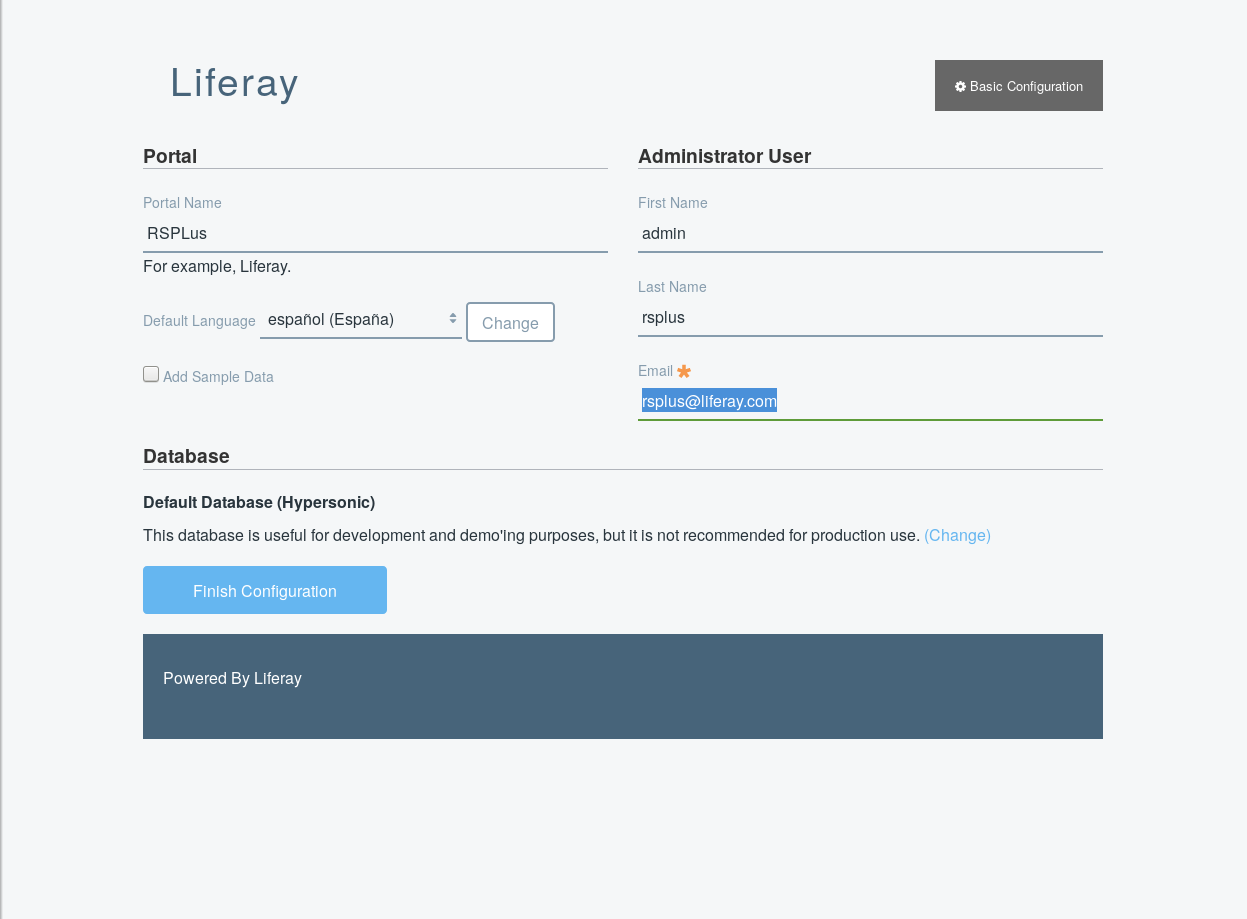
\includegraphics[width=0.8\textwidth]{./img/liferay/1.png}
\end{center}
\caption{Configuración del nombre y del administrador}
\label{img:lr1}
\end{figure}

\par Una vez realizado, pulsar \textit{Finish Configuration} y aceptar las condiciones de uso, así como introducir una contraseña y pregunta de seguridad.

\subsubsection{Configuración de la página base y las subpáginas}
\par Primero se deberá añadir una nueva página pública, tal y como se ve en la imagen \ref{img:lr2}. A continuación, se realiza la configuración inicial (véase la imagen \ref{img:lr3}). Después, se elimina la página inicial tal y como se puede ver en la imagen \ref{img:lr4}. Se procede a crear las subpáginas para \textit{Venta y alquiler} con la opción de añadir la subpágina (véase figura \ref{img:lr5}). Por otro lado, se debe crear una carpeta en Contenidos Web llamada \textit{ComercialesOtrosActivos}, tal y como se puede ver en la imagen \ref{img:lr6}. Tras ello, se debe creae una estructura llamada \textit{OtrosActivos}, como se describe en las imágenes \ref{img:lr7}, \ref{img:lr8}, \ref{img:lr9}.

\par En la estructura, Todos los campos (menos la imagen) deberán ser obligatorios y dependiendo de lo que decida el cliente, se configurarán con unos valores por defecto o no.
